% Based on LLNCS macro package for Springer Computer Science proceedings;
% Version 2.20 of 2017/10/04
\documentclass[runningheads,a4]{llncs}
\usepackage{pre}

\begin{document}

\maketitle

\section{Business Context}
\label{sec:context}
Urban mobility is rapidly evolving, not only due to the increased awareness with
environmental issues, but because of the huge impact digitalization has on the
traditional ways people are able to use transportation systems.

The idea behind \ac{MaaS} is analogous to that of \ac{SaaS}, a term popularized
by Cloud technology: people use the transport network they see better fits their
needs while doing so in a flexible and easy fashion, also enabling the inclusion
of innovative alternatives for personal transportation like rental bike,
scooters, motorcycles, and the likes.

The main challenge arises when it comes to seamlessly integrating all of these
services together without the hassles that come with the need of multiple
ticketing mechanisms or devices, be it through the usage of physical cards or
different mobile applications, proving card/device and fare payment management
arduous tasks.

With this proposal, we aim at building a \ac{MaaS} platform that is capable of
incorporating several transportation services with ease, enabling further
operation adherence in the future, as well as providing the customer a
satisfying experience by removing the need to manage all of the little
intricacies of using multiple different transportation networks.

\section{Entities}
\label{sec:entities}
As part of the proposal, we aim to integrate with three different transportation
operators that provide three equally different means of transportation. We chose
the following operators:
\begin{enumerate*}[label=(\arabic*)]
  \item \ac{ML},
  \item \ac{TTSL}, and
  \item Taxify.
\end{enumerate*}

\subsection{\acl{ML}}
\label{sec:entities.ml}
\acl{ML} is responsible, as the name hints at, for the metropolitan
transportation in Lisbon, enabling users to travel through the city using the
subway. It can be used by acquiring individual tickets, at a fixed fare for
occasional usage. However, for more casual usage, the user can acquire a
monthly subscription.

\subsection{\acl{TTSL}}
\label{sec:entities.transtejo}
\acl{TTSL} is a ferry company operating between Lisbon and regions to the south
side of the river, operating various ships and conventional vessels. It also
provides similar payment models to \ac{ML}'s and can be combined with the latter
as well as with other transportation operators in Lisbon.

\subsection{Taxify}
\label{sec:entities.taxify}
Taxify is an international transportation network company. They're product is an
application that allows users to request a taxi or a private driver from their
smartphone. Unlike the previous services, the fare is computed based on the
distance of the trip.


\section{Services}
\label{sec:services}
The proposed platform is composed of a series of microservices tasked with
different clearly distinguishable goals in order to efficiently perform a
series of actions and participate and relatively elaborate processes which lead
to the 

\subsection{Catalog Management}
\label{sec:services.catalog}
This service is tasked with keeping the set of products, their respective
prices, and usage rules for each of the transportation operators' products,
providing this information as a collection to the other services, or even the
customer, when required.

\subsection{Settlement Distribution}
\label{sec:services.settle}
This service is responsible for registering trip events published by the user
and appropriately distributing the revenue across the operators, taking into
account several aspects that may influence the computation which can be service
dependant, such as the trip's duration.

\subsection{Account Management}
\label{sec:services.account}
This service handles customer related operations. It exposes the \ac{MaaS}
provider’s user registration mechanism, allowing new users to enroll on the
platform; it handles the Product Instantiation, providing a way for users to
purchase "tickets" for their trips and managing the user's finances inside the
system, issuing debit orders and blacklisting the users whose balance prevents
them from using the integrated transportation services.

The aforementioned "tickets" are metaphorical, realized in the way of tokens
with temporal validity the user can then supply to a transportation operator's
validator when using the means of transport the user chose.

\section{Functionality}
\label{sec:functionality}
In order to arrange a system that seamlessly integrates several entities
involved in the \ac{MaaS} ecosystem (Payment services, Transportation services,
Ticketing infrastructure, etc), this system provides a set of crucial
functionalities in order to provide both the users and transportation operators
a good experience.

The system's main selling point, form the user's perspective, is the ability for
the user to use several means of transportation available in the city with ease.
To cope with this requirement, the system provides a catalog with all the
available transportation services and their payment models, allowing the user to
issue a ticket or request a ride on-demand or in advance, in case they won’t
have access to the system at the time of the trip. This process is described in
\Cref{fig:trip}. Another issue that this system addresses is the current
difficulty for users to register in several operators and manage their balance.
The \ac{MaaS} provider replaces the need for multiple accounts spread across the
several operators. Users register once and can check the balance and history of
their account. The user registration process is illustrated in
\Cref{fig:new-user}.

When it comes to transportation operators, this system facilitates the
integration of new ones, allowing them to register and announce their products.
Since the handling of check-in and check-out events belongs to \ac{MaaS}
provider, the operators don’t need to implement any logic related to settlements
or user identity verification. A process that entails these aspects is depicted
as a \acs{BPMN} model in \Cref{fig:trip}. The \ac{MaaS} provider supports
several payment models, providing compatibility with already adopted
transportation services.


\begin{sidewaysfigure}
  \centering
  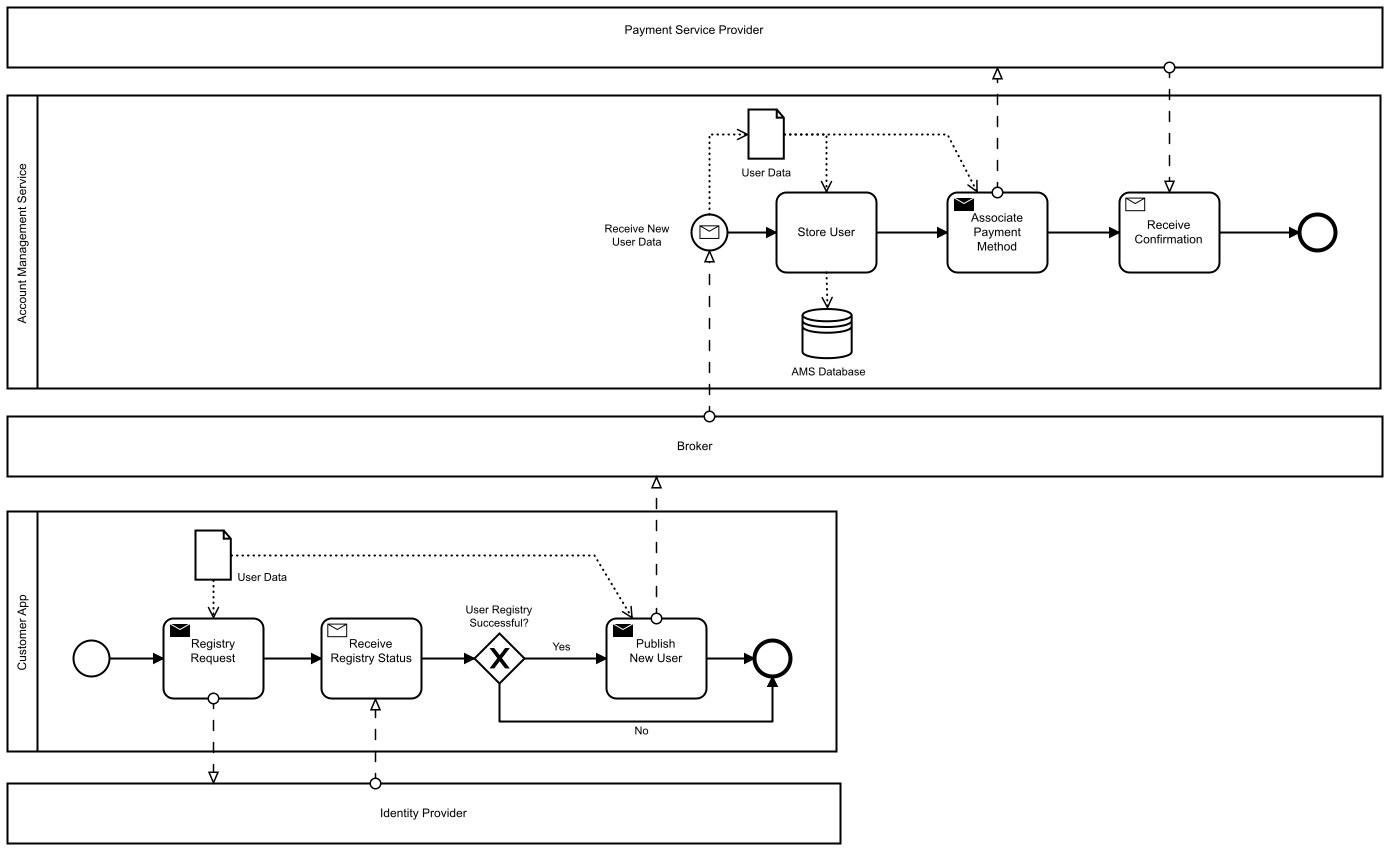
\includegraphics[width=.8\paperwidth]{img/new-user.png}
  \caption{User registration process}
  \label{fig:new-user}
\end{sidewaysfigure}
\begin{sidewaysfigure}
  \centering
  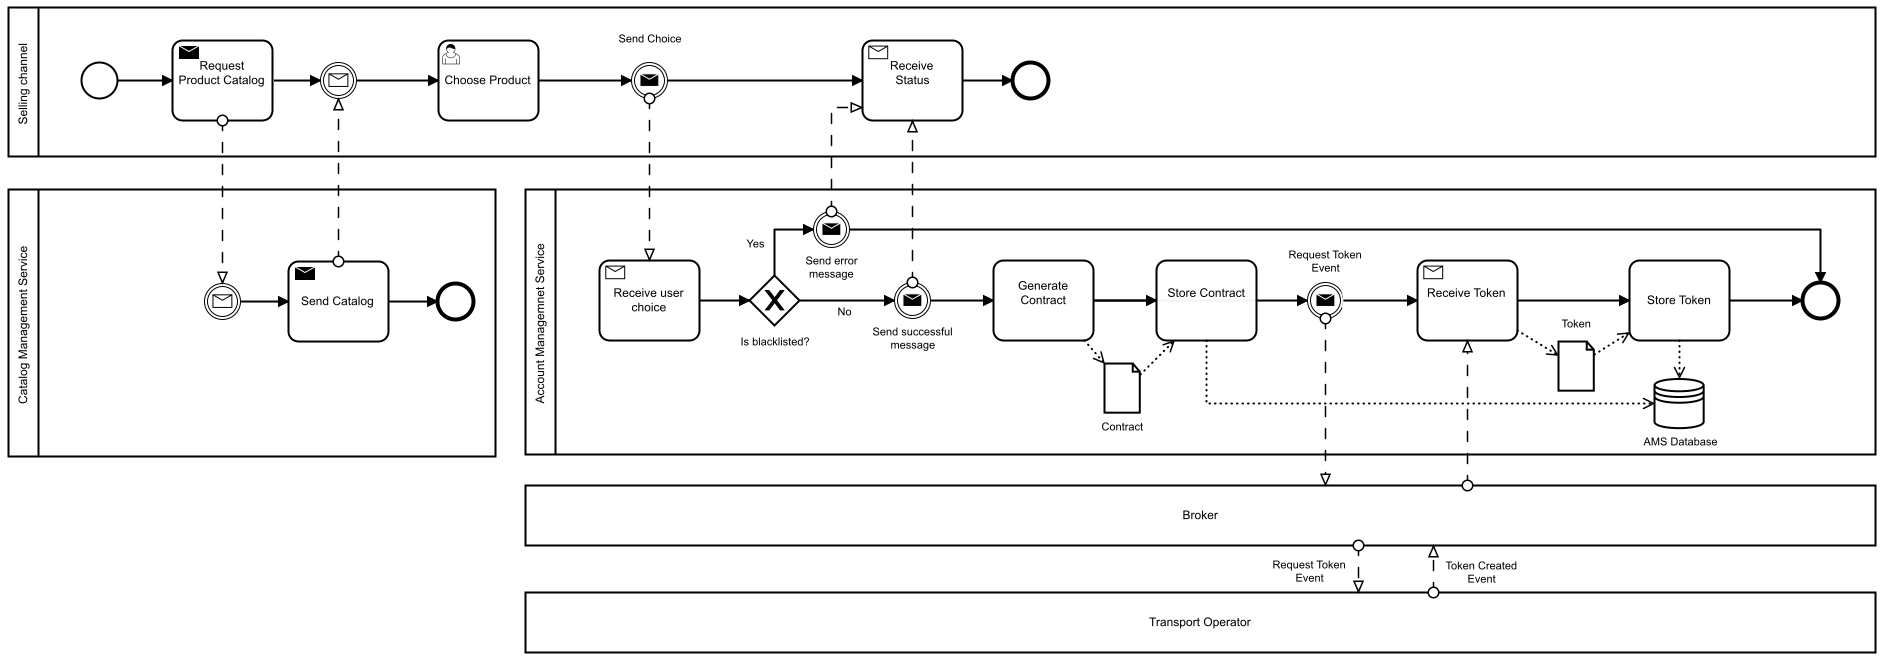
\includegraphics[width=.8\paperwidth]{img/purchase-product.png}
  \caption{Product purchase}
  \label{fig:purchase-product}
\end{sidewaysfigure}
\begin{sidewaysfigure}
  \centering
  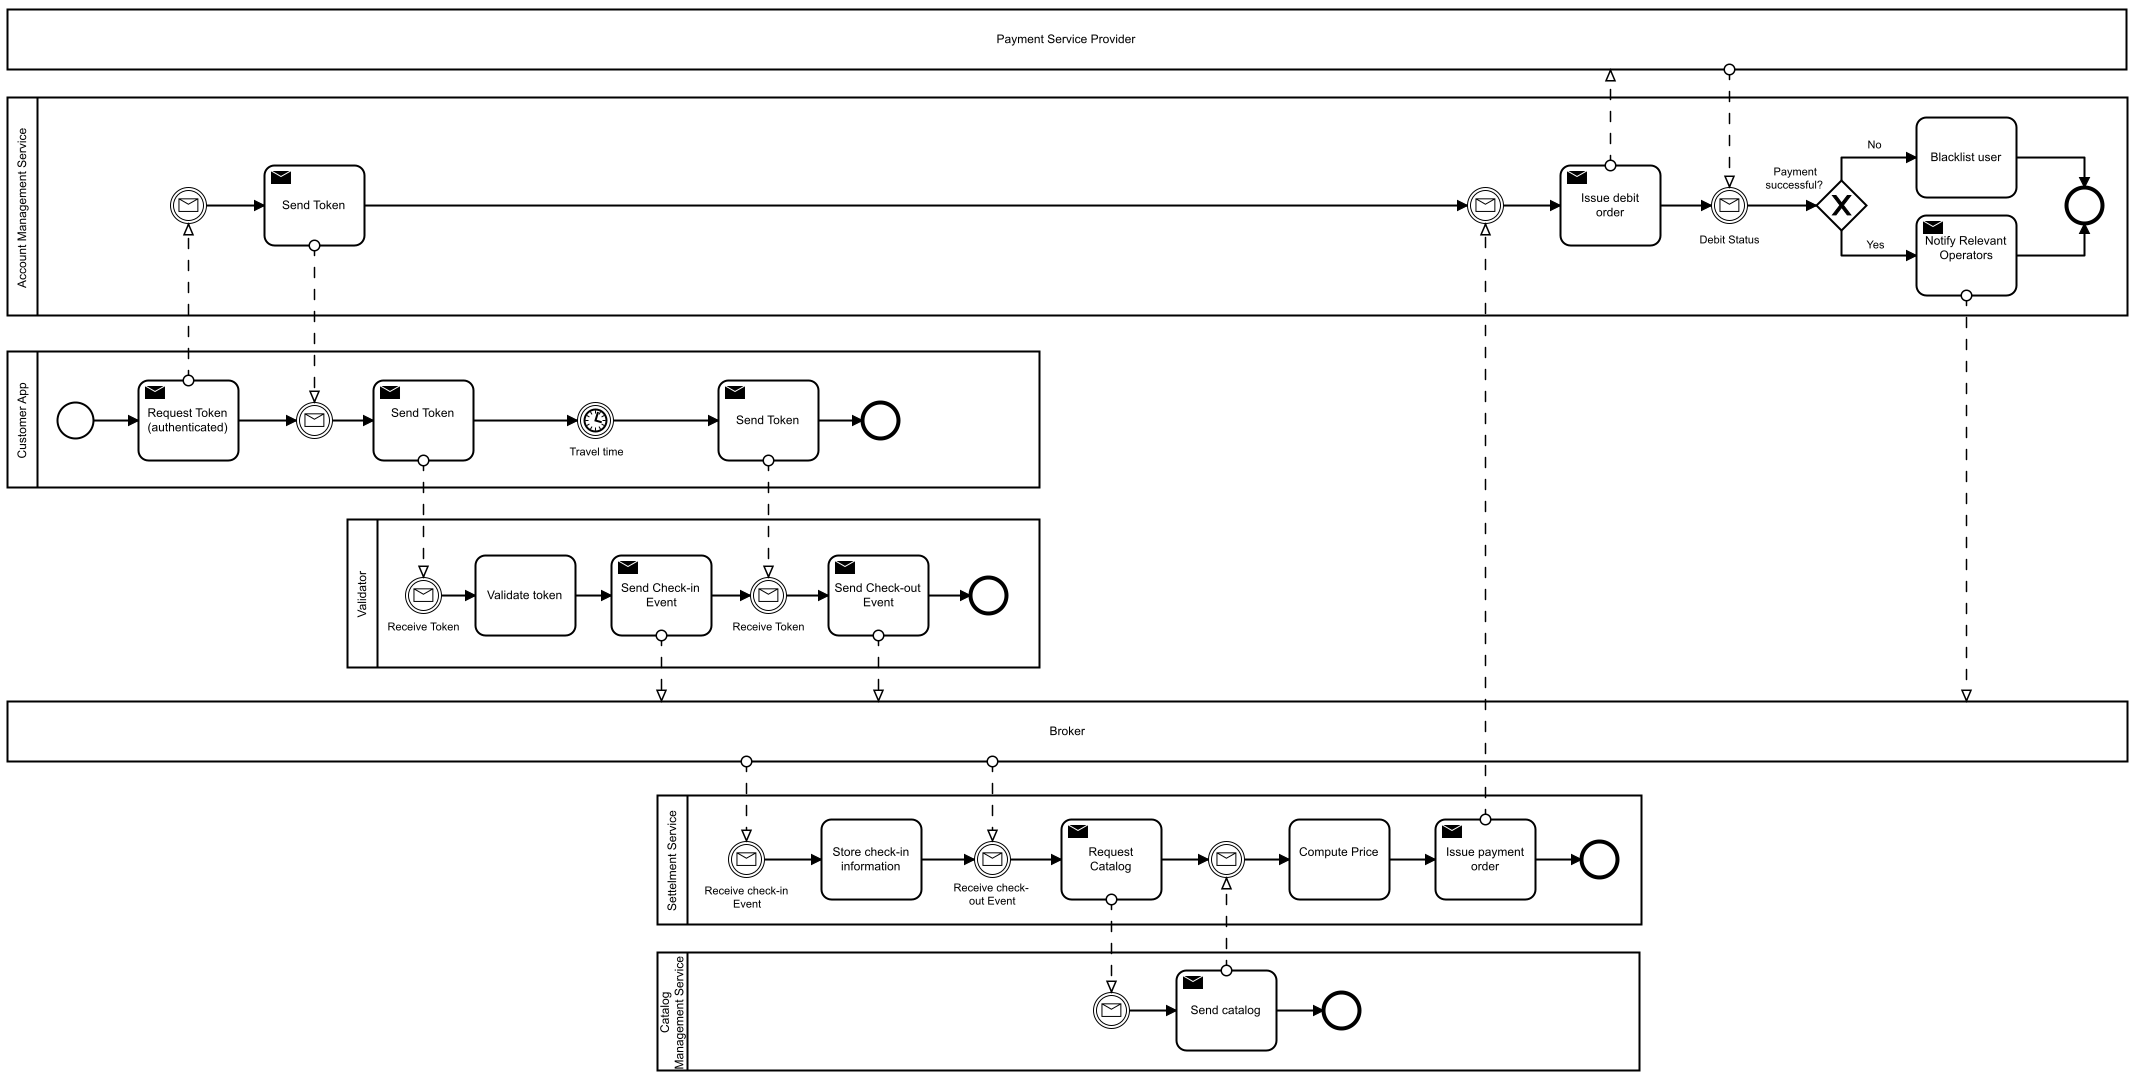
\includegraphics[width=.8\paperwidth]{img/trip.png}
  \caption{Check-in / Check-out trip process}
  \label{fig:trip}
\end{sidewaysfigure}


\begin{acronym}
  \acro{BPMN}{Business Process Model and Notation}
  \acro{MaaS}{Mobility as a Service}
  \acro{ML}{Metro de Lisboa}
  \acro{SaaS}{Software as a Service}
  \acro{TTSL}{Transtejo \& Soflusa}
\end{acronym}
\end{document}
